\def\year{2016}
%File: formatting-instruction.tex
\documentclass[letterpaper]{article}
\usepackage[ruled,vlined,linesnumbered]{algorithm2e}
\usepackage{aaai}
\usepackage{times}
\usepackage{helvet}
\usepackage{color}
\usepackage{graphicx}
\usepackage{courier}
\usepackage{amsthm}
\usepackage{amsmath}
\usepackage{amssymb}
\usepackage{natbib}
\usepackage{url}

\newcommand\note[1]{\textcolor{red}{#1}}
\newcommand\comment[1]{}


% Defs 
%\newcommand{\public}[1]{\textit{public(#1)}}
%\newcommand{\private}[2]{\textit{private_{#1}(#2)}}
\newcommand{\private}{\textit{private}}
\newcommand{\eff}{\textit{eff}}
\newcommand{\pre}{\textit{pre}}
\newcommand{\delete}{\textit{delete}}
\newcommand{\public}{\textit{public}}
\newcommand{\false}{\textit{false}}
\newcommand{\true}{\textit{true}}
\newcommand{\init}{\textit{init}}
\newcommand{\load}{\textit{load}}
\newcommand{\unload}{\textit{unload}}



\frenchspacing
\setlength{\pdfpagewidth}{8.5in}
\setlength{\pdfpageheight}{11in}



\pdfinfo{
/Title (Privacy Preserving LAMA)
/Author (Shlomi Maliah, Guy Shani, Roni Stern)}
\setcounter{secnumdepth}{0}  

\newtheorem{definition}{Definition}
\newtheorem{theorem}{Theorem}
\newcommand\roni[1]{\textcolor{blue}{roni: #1}}
\newcommand\guy[1]{\textcolor{red}{guy: #1}}
\newcommand\cprivacy{object cardinality privacy}

\theoremstyle{definition}
\newtheorem{example}{Example}[section]
\nocopyright

\setcounter{secnumdepth}{2}

 \begin{document}
% The file aaai.sty is the style file for AAAI Press 
% proceedings, working notes, and technical reports.
%
\title{Privacy Preserving LAMA}
\author{Shlomi Maliah \and Guy Shani \and Roni Stern\\\\
Ben Gurion University of the Negev, Israel\\
}
%\author{Shlomi Maliah \and Guy Shani \and Roni Stern \\
%Association for the Advancement of Artificial Intelligence\\
%2275 East Bayshore Road, Suite 160\\
%Palo Alto, California 94303\\
%}
\maketitle

\begin{abstract}
\begin{quote}
%Collaborative privacy preserving planning (CPPP) is a recently introduced setting in which multiple agents collaborate to achieve a goal, keeping certain facts about the world private. A prominent approach in the development of CPPP algorithms is to use various components from single agent planning algorithms and adapt them while preserving privacy. In this short paper, we show how the components of LAMA, arguably one of the most successful single-agent planners, can be used in a privacy preserving manner. These components include alternating between a landmark heuristic and an FF heuristic, preferred operators and deferred heuristic evaluation. We integrate the components into the Greedy Privacy Preserving Planner, a state-of-the-art CPPP algorithm. The resulting algorithm performs better than other CPPP algorithms from the recent Competition of Distributed and Multiagent Planners. 
In collaborative privacy preserving planning (CPPP), multiple agents collaborate to achieve a goal while keeping certain facts about the world private. A prominent approach in the development of CPPP algorithms is to use components from single agent planners and adapt them to preserve privacy. In this short paper, we show how the components of LAMA, arguably one of the most successful single-agent planners, can be used in a privacy preserving manner. These components include alternating between a landmark heuristic and an FF heuristic, preferred operators and deferred heuristic evaluation. We integrate the components into the Greedy Privacy Preserving Planner, a state-of-the-art CPPP algorithm. The resulting algorithm performs better than other CPPP algorithms from the recent Competition of Distributed and Multiagent Planners. 
\end{quote}
\end{abstract}

%\vspace{-0.1cm}
\section{Introduction}

% Motivation: CPPP is so important. 
% TODO: Can shorten significantly
Collaborative privacy preserving planning (CPPP) is a recently introduced setting in which multiple agents cooperate to achieve joint goals while concealing certain facts. As a motivating scenario, consider an army organization outsourcing its food supply to external caterers. Caterers unloads packaged food in logistics center and army trucks deliver the packages to the various bases. The army and the caterer must plan together to deliver appropriate amounts of food to the army bases, but the army may not wish to discloser to the caterers the location of its bases or the number of soldiers in each base. %, or the number of soldiers on each base, to be disclosed to the caterers. %The caterer may not want the army to be aware of the number of trucks it operates.%to the various logistic centers at the right time, while not disclosing the number and location of the bases, as well as the number of trucks owned by .
%Even though the caterers and the army operate jointly to provide food to the army bases, the army may not wish the location of these bases, or the number of soldiers on each base, to be disclosed to the caterers. The caterer may not want the army to be aware of the number of trucks it operates. One possible solution is to use logistics centers, where the caterer unloads packaged food, and the army trucks then deliver the packages to the various bases. The army and the caterer must plan together to deliver appropriate amounts of food to the various logistic centers at the right time, while not disclosing the number and location of the bases, as well as the number of trucks.


% We use the MA-STRIPS formalism. 
% It is so popular and there is even a competition
\cite{brafman2013complexity} proposed an attractive framework for such planning problems called multi-agent STRIPS (MA-STRIPS), which has attracted much attention in recent  years~\citep{tozicak2015onInternally,torreno2015global,vstolba2014relaxation,maliah2014privacyPreserving}. The first Competition of Distributed and Multiagent Planners (CoDMAP), held last year, already featured many planners from 10 different groups~\cite{vstolba2015competition}. 
% Common approach: take single agent algorithms and make them privacy aware.
% We follow this approach in making PP-LAMA
Many successful CPPP algorithms borrow or adapt algorithmic components from the single-agent planning literature. For example, privacy preserving versions have been proposed for popular single-agent heuristics such as landmarks~\citep{maliah2014privacyPreserving,torreno2015global,vstolba2015admissible}, FF~\citep{vstolba2014relaxation}, and pattern databases~\citep{maliah2015privacy}. In this short paper we propose a CPPP algorithm that successfully adapts and uses key components of LAMA~\citep{richter2010lama}, a renowned single-agent planner. 

% LAMA, is great. It uses LM, FF, preferred operators and deferred heuristic evaluation
LAMA is perhaps one of the most successful single-agent planners. 
% Say something about the ICP it has won
It uses a forward heuristic search algorithm employing both a landmark-based heuristic~\citep{richter2008landmarks} and the FF delete-relaxation heuristic~\citep{hoffmann2001ff}, and alternates between them~\citep{roger2010theMore}. In addition, LAMA introduced preferred operators and deferred heuristic evaluation~\citep{richter2009preferred}, which are both common components in state-of-the-art single-agent planning algorithms. 

% We make a PP-LAMA in GPPP. It rocks!
The main contribution of this work is in the integration of these components into the Greedy Privacy Preserving Planner (GPPP)~\citep{maliah2014privacyPreserving}, a state-of-the-art CPPP algorithm. Experiments with the CoDMAP benchmarks show that the resulting algorithm, which we call PP-LAMA, outperforms all previous CPPP algorithms. 
% In doing so, we had to develop new PP stuff
Some LAMA components were already adapted to preserve privacy by prior work. \cite{vstolba2014relaxation} and \cite{maliah2014privacyPreserving} 
proposed a privacy preserving versions of the FF and landmark heuristics, and \cite{torreno2015global} proposed alternating multiple heuristics. 
We explain how the other components of PP-LAMA operate in a way that preserves privacy. 
In particular, we highlight the importance of deferred heuristic evaluation, which is especially useful for reducing the collaborative effort in computing privacy preserving heuristics. Moreover, we improve on the landmark detection algorithm used by \cite{maliah2014privacyPreserving}, showing a simple modification that allows finding substantially more landmarks. %and propose a way to detect the same of landmarks as detected by the single agent landmark detection algorithm, thus resulting in a better landmark-based heuristic. 

%domains used by the CoDMAP
%t alternates between  queues ordethese heuristic, as well as a queue containing states generated by {\em preferred operators} 
%alternates between multiple priority queues to choose which state to expand next,  In this short paper we integrate various components of LAMA into the Greedy Privacy Preserving Planner (GPPP)~\cite{maliah2014privacyPreserving}. The resulting privacy preserving planner is called PP-LAMA. Some of the components of PP-LAMA were already introduced in previous work, while other components are novel. Specifically, PP-LAMA has the following LAMA-based improvement over GPPP: (1) an improved privacy preserving landmark detection algorithm able to find all landmarks as in the single agent case, (2) alternating this heuristic with a privacy preserving version of  FF introduced by \cite{vstolba2014relaxation}, (3) used preferred operators and deferred node evaluation. 
%The contribution of this work is three-fold. First, in the improved landmark detection algorithm. Second, a privacy preserving way to implement preferred operators and lazy node geneartion. Third, we integrate all this improvements into PP-LAMA and show that it outperforms all other planners over the CoDMAP problems. In addition, we observe that the deferred heuristic lazy evaluation of LAMA is especially useful for the time consuming collaborative effort in computing the privacy preserving FF heuristic.


%method heuristic in the adaption of preferred operators  describe a better landmark

%adaptation of various components of LAMA into a privacy preserving setting and integrate them in a single, highly effective, privacy preserving planner. Specifically, we focus on the following LAMA components:

%the landmark computation mechanism, the FF heuristic, and preferred operators. Our landmark identification improves upon previously suggested privacy preserving landmark identification approaches, obtaining the same set of landmarks as LAMA would identify when ignoring the privacy constraints. The deferred heuristic lazy evaluation of LAMA is especially useful for the time consuming collaborative effort in computing the privacy preserving FF heuristic.




%In an effort to take advantage of the success of single agent planning algorithms, various algorithmic components of 

%A popular and successful approach is based on forward heuristic search~\cite{nissim2014distributed,maliah2015privacy,maliah2014privacyPreserving,vstolba2014relaxation,vstolba2015admissible}. Several  heuristics have been suggested for this task, including an adaptation of the FF heuristic \cite{vstolba2015admissible} and landmarks \cite{maliah2014privacyPreserving}. 

%In classical planning it is widely agreed that landmarks --- logic formulas that must occur on every path to goal --- provide a good, yet partial, estimate for the distance to the goal \cite{richter2008landmarks}. Indeed, landmarks are typically combined with other heuristics in order to achieve a competitive performance in heuristic search. Specifically, the LAMA planner \cite{richter2010lama} combines landmarks with the FF heuristic \cite{hoffmann2001ff} to achieve an impressive performance on classical planning benchmark domains.

%In this short paper we provide an adaptation of LAMA into a privacy preserving setting, which we call PP-LAMA. We explain the various components of PP-LAMA --- the landmark computation mechanism, the FF heuristic, and preferred operators. Our landmark identification improves upon previously suggested privacy preserving landmark identification approaches, obtaining the same set of landmarks as LAMA would identify when ignoring the privacy constraints. The deferred heuristic lazy evaluation of LAMA is especially useful for the time consuming collaborative effort in computing the privacy preserving FF heuristic.

%We provide experiments on benchmarks form the latest CoDMAP competition, showing PP-LAMA to solve more problems than any other privacy preserving planner.

%\vspace{-0.1cm}
\section{Background}

We now briefly describe the privacy preserving planning setting, the heuristics used by LAMA, and the GPPP algorithm. 

%and the classical landmark identification and FF heuristics.

\subsection{Privacy Preserving Planning}

\begin{figure}
\centering
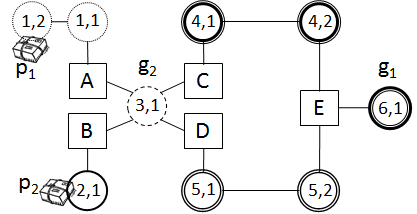
\includegraphics[scale=0.5]{Logistics}
\label{fig:logistics}
%\caption{A logistics example, where trucks deliver packages between logistics centers, denoted by squares. Each agent covers a set of cities, denoted by circles, and labeled $i,j$ where $i$ is the agent covering the city and $j$ is the local city index. The logistic centers can be entered by several agents, serving as collaboration sites.}
\caption{A logistics example.}
%\vspace{-0.5cm}
\end{figure}

% MA-STRIPS
An MA-STRIPS problem~\citep{brafman2013complexity} is represented by a tuple $\langle P, \{A_i\}_{i=1}^k, I ,G \rangle$ where $k$ is the number of agents, $P$ is a finite set of facts (can be true of false), $A_i$ is the set of actions agent $i$ can perform, $I$ is the start state, and $G$ is the goal condition.	
%\begin{itemize}
%	\item $k$ is the number of agents
%	\item $P$ is a finite set of facts (can be true of false). 
%    \item $A_i$ is the set of actions agent $i$ can perform. 
%	\item $I$ is the start state.
%	\item $G$ is the goal condition.	
%\end{itemize} 
Each action $a=\langle \pre(a), \eff(a) \rangle$ is defined by its preconditions ($\pre(a)$), and effects ($\eff(a)$). Preconditions and effects are logical formulas over $P$. A state is a conjunction of facts in $P$ (true or false). The goal $G$ is also a conjunction of facts. 
A solution is a {\em plan} that achieves $G$, i.e., a sequence of actions transforming the initial state ($I$) to a state that satisfies $G$. % the goal condition ($G$). 
%The result of applying an action $a$ to a state $s$ is denoted by $a(s)$. A solution is a {\em plan} $\pi$=($a_1,\ldots,a_k$) such that $G\subseteq a_k(\ldots(a_1(I)\ldots)$, i.e., a sequence of actions transforming the initial state ($I$) to a state satisfying the goal condition ($G$). 
%\roni{Shouldn't this be a_k(\ldots(a_1(I)\ldots) \models G ?}


% Privacy in MA-STRIPS
Privacy-preserving MA-STRIPS extends MA-STRIPS by defining sets of variables and actions as private, known only to a single agent. Formally, 
a privacy-preserving MA-STRIPS problem defines a set of facts as public, denoted $\public(P)$, and a set of actions as public, where $\public_i(A) \subset A_i$ are the public actions of agent $i$. 
%$\public(P)$ is the set of public facts in $P$, and $\public_i(A) \subset A_i$ is the set of public actions of agent $i$. 
It is assumed that when a public action is executed, all agents are aware of the execution, and view the public effects of the action. 
A privacy-preserving MA-STRIPS problem also defines for each agent $i$ a set of facts and actions as private, denoted by $\private_i(P)$ and $\private_i(A)$, respectively. The identity of the private facts and actions must not be revealed to the other agent during planning and during execution. The public and private facts of each agent are disjoint, i.e., $\private_i(P)\cap \public(P)\emptyset$, and the union of the public facts and all private facts form the entire set of facts in the underlying MA-STRIPS problem, i.e., $\bigcup_{i=1}^k \private_i(P) \cup \public(P)=P$.

For ease of exposition we assume that all goals are public.
% A solution to a CPPP problem, a valid high-level plan
A solution to a privacy-preserving MA-STRIPS problem, is a sequence of public and private actions. We say that the sequence of public actions in such a solution is a high-level, or public, plan that must be extended to a full plan using private actions of various agents. A high-level plan is said to be {\em valid} if each agent can plan independently to achieve the private preconditions on the public actions it executes in the high level plan \cite{maliah2014privacyPreserving}.

% Example
Figure~\ref{fig:logistics} illustrates a simple logistic example in which the agents are trucks tasked with delivering packages. The set of facts $P$ represents the location of the two packages and six trucks. Each truck has three actions: move, load, and unload, corresponding to moving the truck between locations, loading a package and unloading it. 
%Trucks can only drive along the edges in Figure~\ref{fig:logistics}. 
%Agents are heterogeneous  and their range is restricted: location $i,j$ can only be reached using truck $i$. Rectangles are logistic centers, which are reachable by all trucks. % visited by multiple trucks that load or unload packages. 
Each truck is owned by a different company and may have different areas of operation, and no company wants to share its location and coverage (which locations it can reach) with other companies. Thus, all the facts representing the location of trucks are private, while the facts representing whether a package is at a logistic center are public. Only the load/unload actions at the logistic centers are public, while the move actions are private for each agent, as well as loading and unloading packages at private locations.  


% RONI: We said all this about LAMA in the introduction. No information is really added here.
%\subsection{LAMA}

% LAMA is great. It uses search with heuristics
%LAMA is a single-agent classical planning algorithm, which has repeatedly demonstrated strong performance in planning competitions~\cite{richter2010lama}. Due to lack of space, we provide here a very brief review of LAMA, avoiding many details. LAMA uses heuristic search, with two different heuristics --- a {\em landmark} heuristic and the {\em FF heuristic}. The heuristics are maintained in separate open lists, and the search alternates in selecting which node to expand from the lists. Next, we describe the main components of LAMA, which are relevant for PP-LAMA. 

\subsection{Landmark Heuristics}
Landmarks, as used in LAMA, % Roni: I added this to avoid complaints about ignoring action landmarks
are propositional formulas that must be hold at some point during the execution of every successful plan~\citep{richter2008landmarks}. A landmark heuristic function evaluates a state by considering the number of landmarks that still needs to be achieved. A popular method for identifying landmarks searches backwards from the goal. At each phase, one landmark is selected for development. All actions that can satisfy this landmark are identified, and a new landmark is constructed from their preconditions. When all these actions share a single fact, that fact is identified as a new landmark. Otherwise, a disjunctive formula is created from some facts that appear in the actions preconditions. When developing a landmark, all actions that take facts in this landmark as preconditions are ignored, in order to avoid circular reasoning.

\subsection{The Fast Forward (FF) Heuristic}
The FF heuristic begins by computing the relaxed planning graph, where facts are organized into layers, and all edges are between consecutive layers~\citep{hoffmann2001ff}. The first layer contains all the facts that hold at the current search state. To construct the next layer the FF heuristic considers the actions that can be executed at the current state, i.e., the actions whose preconditions are satisfied by the facts in the current layer. The next layer in the relaxed planning graph consists all the facts in the previous layer and all the facts that are effects of these set of actions. Importantly, {\em delete effects}, i.e., effects that remove facts from the state, are ignored. A result of ignoring delete effects 
is that once an action has participated in the construction of a layer, there is no need to consider it in the construction of future layers. For each fact $p$, the FF heuristic maintains the action $a_p$ that has achieved it for the first time. Then, it constructs an edge between the preconditions of $a_p$ on the previous level and $p$. After the graph construction, FF computes a plan over the relaxed graph, starting from the goal and moving backwards: first considering the goal facts and adding all the actions that achieved them to the plan. Then considering the preconditions of these actions, and so forth, ignoring repeated facts.

%\vspace{-0.1cm}
\subsection{GPPP}

%Like LAMA, the GPPP algorithm~\cite{maliah2014privacyPreserving} is a heuristic best-first privacy preserving planner. 

The GPPP algorithm~\citep{maliah2016collaborative} is a CPPP algorithm based on heuristic forward search. %best-first search. 
%heuristic best-first privacy preserving planner. 
The first phase in GPPP is the {\em high-level planning} phase, in which the agents collaboratively perform a best-first search on a relaxed version of the CPPP problem in which only public actions are used. To maintain privacy, states in this search are represented by the set of public facts that hold for that state, and a set of private state identifiers, one for each agent. Every agent can map its private identifiers to a set of private facts. 
When a state $s$ is expanded, each agent generates new states by applying the public actions it can execute in $s$. In addition to the effects of the executed public action, the generated state also includes all private facts that the corresponding agent can achieve by applying private actions and using delete relaxation~\citep{hoffmann2001ff}. 
%Each agent estimates, using delete relaxation~\citep{hoffmann2001ff}, which private facts it could achieve following a public action execution, and which public actions can now be executed given these private facts. 
% TODO-R: The term high-level public plan may be unclear
The high-level planning phase ends when a high-level public plan has been found that enables achieving all goals. Then, all agents compute private plans to achieve the preconditions of the public actions in the high level public plan. If some agent cannot achieve the preconditions of one of its actions in the high-level plan then this second phase fails then the high level planning phase resumes.

%Once a high-level public plan has been found that enables achieving all goals, all agents compute private plans to achieve the preconditions of the public actions in the high level public plan. If this phase fails, because some agent cannot achieve the preconditions of a public action, then the high level search continues.

%After each state expansion, all agents report whether they can reach all goals given the expanded states. As GPPP estimates states using delete relaxation, even if the agents report that all goals can be achieved, the public plan that achieves them may not be sound. Thus, once a public plan has been achieved, the agents compute private plans to achieve the preconditions of the public actions in the high level plan. If this phase fails, because some agent cannot achieve the preconditions of a public action, then the high level search continues.


%The algorithm begins by searching for a high-level public plan. The algorithm maintains a global queue of states to expand, where each state is represented by the set of public facts that hold for that state, and a set of private state identifiers, one for each agent. Every agent can map its private identifiers to a set of private facts.

%GPPP uses only public actions to expand the current state. Every time a state is expanded, all agents participate in computing the expanded state. Each agent estimates using delete relaxation which private facts it can achieve following the public action execution, and which public actions can now be executed given these private facts. 

\cite{maliah2014privacyPreserving} show that GPPP's efficiency depends on the heuristic function used to guide the high-level search and that effective heuristics can be computed by a collaborative effort of the agents. For example, collaboratively computing a landmark heuristic requires each agent to reports the number of landmarks satisfied in a state. Using such heuristic allowed GPPP to show impressive performance, but the need to collaborate for evaluating the heuristic of each expanded state slows down the search process considerably. 
This is especially problematic for the FF heuristic, which requires agents to collaboratively find a relaxed plan.  
%For example, the privacy-preserving FF heuristic requires agents to coleach agent needs to recompute its relaxed plan reports the number of landmarks satisfied in a state. Using such heuristic allowed GPPP to show impressive performance, but the need to collaborate for evaluating the heuristic of each expanded state slows down the search process considerably. 
Our PP-LAMA algorithm builds upon GPPP and is especially suited to address this limitation by borrowing from LAMA the preferred operators and deferred heuristic evaluation techniques (Section~\ref{sec:preferredOperators}). 

%to specifically address this limitation. 
%. The main changes in PP-LAMA are the use of multiple queues, and the lazy heuristic estimation.
%This motivated this work, in which preferred operators and deferred heuristic evaluation are borrowed from LAMA to specifically address this limitation.  

%Although GPPP has shown impressive coverage, the need to collaborate for evaluating the heuristic of each expanded state slows down the search process considerably.

%After each state expansion, all agents report whether they can reach all goals given the expanded states. As GPPP estimates states using delete relaxation, even if the agents report that all goals can be achieved, the public plan that achieves them may not be sound. Thus, once a public plan has been achieved, the agents compute private plans to achieve the preconditions of the public actions in the high level plan. If this phase fails, because some agent cannot achieve the preconditions of a public action, then the high level search continues.

%\vspace{-0.1cm}
\section{Privacy Preserving LAMA}
%\vspace{-0.3cm}
\begin{algorithm}[htb]
\footnotesize
	\SetKwBlock{PPLAMA}{PP-LAMA()}{end}
\PPLAMA{
	%\KwIn{$\pi_i$, the local view of agent $i$}
  	%\KwOut{$P_{full}$, a complete plan} 
    
    Init all open lists to hold the initial state\\
%    $c_{pref} \leftarrow 1$; ~ $c_{\overline{pref}} \leftarrow 0$;~     $turn \leftarrow 1$\\
    $c_{LM} \leftarrow 0$;     $c_{FF} \leftarrow 0$;     $c_{pLM} \leftarrow 0$;     $c_{pFF} \leftarrow 0$;\\
    
    
%    ~ $c_{\overline{pref}} \leftarrow 0$;~     $turn \leftarrow 1$\\
   
    \While{some open list is not empty}{
    	{\em active-list}$\gets$ {\bf ChooseList}($c_{LM}$,$c_{FF}$,$c_{PLM}$,$c_{pFF}$) \nllabel{line:chooseList}\\    	
        $s \leftarrow $ best state in {\em active-list}\\
        Remove $s$ from all open lists\\
        \If{$s \models G$}{
        	$P_{pub}\leftarrow $ the public plan to achieve $s$\\
        	$P_{full}\leftarrow$ private extensions for $P_{pub}$ \nllabel{line:extend}\\
            \If{$P_{full}$ is valid}{
            	\Return $P_{full}$\\
            }
        }
        Find achievable private facts in $s$ \nllabel{line:findAchievable} \\
        Compute all heuristic values for $s$ \nllabel{line:h}\\
	\If{$s$ was generated by a PO and h($s$) is the lowest so far for either FF or LM}{
%\If{for either FF or LM, h($s$) is the lowest so far}{
        	$c_{pLM}$$\gets$$c_{pLM}+1000$; $c_{pFF}$$\gets$$c_{pFF}+1000$ \nllabel{line:boosting}\\
        }
        \Else{
        	$c_{LM}\gets c_{LM}+1$; $c_{FF}\gets c_{FF}+1$\\
        }
        \ForEach{public action $a_{pub}$ applicable in $s$}{
            $s' \leftarrow apply(s, a_{pub})$ \nllabel{line:generate} \\
            \If{$a_{pub}$ is a preferred operator for $s$}{
                Add $s'$ into all open lists w. $h(s)$ \nllabel{line:deferred1}\\
            }
            \Else{
	            Add $s'$ into FF and LM open lists w. $h(s)$ \nllabel{line:deferred2}\\    
            }
        }    
    }


}
\caption{The PP-LAMA algorithm} 
\label{alg:PP-LAMA}
\end{algorithm}
%\vspace{-0.1cm}

Next, we present PP-LAMA, starting by describing its different components. %: an improved privacy-preserving landmark heuristic, a privacy preserving FF heuristic, preferred operators and deferred heuristic evaluation. 

%--- a privacy preserving LAMA implementation. We begin by describing the privacy preserving landmark identification mechanism, and then the privacy preserving FF heuristic computation. Finally we describe the privacy preserving LAMA algorithm itself.

\subsection{Privacy Preserving Landmark Detection}
% We are based on us
We use the landmark identification process of \cite{maliah2014privacyPreserving}, where agents collaborate in identifying landmarks, and augment it with an improved detection of private landmarks. 
% The process from a bird's eye perspective. 
The process begins by adding each fact (or disjunction of facts) in the goal as a landmarks. Then, the agents agree on a landmark and {\em develop} it, potentially adding more landmarks. This process continues until there are no more landmarks to develop. 
% Developing a landmark: find achievers, get new LM from their preconditions
{\em Developing} a landmark $\phi$ means checking which actions can achieve $\phi$, and then considering the preconditions of these actions as additional landmarks. 
To identify which actions achieve $\phi$, the agents first check which facts they can achieve without requiring any facts in $\phi$. 
This is done effectively by ignoring the delete effects of agents' actions (i.e., using a delete-relaxation), applying them iteratively (starting from the initial state) and sharing the achieved public facts between the agents. Then, each agent considers which actions it can perform to achieve facts in $\phi$ given this set of achieved facts. The preconditions of these actions form a new landmark. 

% Keeping privacy
% Q1: For a landmark a OR b, 
% if b is private, and has a single achiever with a single precondition c
% what would be the generated landmark: a OR c ??

A landmark $\phi$ can be a disjunction of public and private facts: $\phi=\public(\phi)\vee \phi_1,\ldots,\phi_k$, 
where $\public(\phi)$ is the public facts in $\phi$ and $\phi_i$ are the private facts of agent $i\in[1,\ldots,k]$ in $\phi$. 
Each agent develops its private facts in $\phi$ and all agents develop together the public facts. Formally, if
 $d(\phi)$ denoted developing a landmark $\phi$ then, $d(\phi)=d(\public(\phi))\vee d(\phi_1) \vee \dots d(\phi_k)$. 
%Each agent develops its private facts in $\phi$ and all agents develop together the public facts. Importantly, if $\phi_i$ is the private facts of agent $i$ in $\phi$ and $\phi_i'$ is the facts developed from $\phi_i$, then the landmark developed from $\phi$ is $\vee_{i=1}^k \phi_i'$. 
To preserve privacy, only the public facts are published to the other agents. For private facts, all agents agree on a unique ID for this landmark, and each agent maintains a mapping from this ID to its own set of private facts that participate in this landmark. 
Our landmark identification process improves on that of \cite{maliah2014privacyPreserving} in that it allows detecting and developing landmarks that contain private facts of multiple agents. Experimentally, this improvement allows finding more than twice as many landmarks in some domains from the CoDMAP centralized planning track~\cite{vstolba2015competition}. 


The detected landmarks are used to evaluate a state during planning. Each agent publishes which landmarks it identified as satisfied in the state. The number of landmarks that at least one agent can satisfy is used as the landmarks heuristic estimate for that state. We refer to this heuristic as LM. 

%LM-GPPP allowed only for landmarks with private facts of a single agent.




%For private facts, all agents agree on a unique ID for this landmark, and each agent maintains a mapping from this ID to its own set of private facts that participate in this landmark. 
%are shared between the agents can contain private and public facts, it is represented like states in the high-level planning of GPPP: the The key innovation is that instead of 

%using the published set of public facts, all agent develop the landmark backwards, obtaining a new landmark. Each agent develops its own private parts of the landmark, and all agents develop together the public parts of the landmark. This landmark, again, can be composed of public and private facts. Only the public facts are published to the other agents. For private facts, all agents agree on a unique ID for this landmark, and each agent maintains a mapping from this ID to its own set of private facts that participate in this landmark. 


% How landmarks look like
%Landmarks may contain private and public facts. To preserve privacy, only the public facts in a landmark is shared between the agents. To preserve the private facts in that landmark, all agents agree on a unique ID for each landmark, and each agent maintains a mapping from this ID to its own set of private facts that participate in this landmark.


%The process begins with all agents agreeing on a landmark to develop. This landmark can be a public fact, a private fact, or a disjunction of public and private facts. All agents then compute iteratively the set of public facts that can be achieved, avoiding actions that have the landmark facts as preconditions, to avoid circular reasoning.

%Then, using the published set of public facts, all agent develop the landmark backwards, obtaining a new landmark. Each agent develops its own private parts of the landmark, and all agents develop together the public parts of the landmark. This landmark, again, can be composed of public and private facts. Only the public facts are published to the other agents. For private facts, all agents agree on a unique ID for this landmark, and each agent maintains a mapping from this ID to its own set of private facts that participate in this landmark. 




\subsection{Privacy Preserving FF}
\begin{table*}
\begin{tabular}{cc}
    \begin{minipage}{.45\textwidth}
    \resizebox{\textwidth}{!}{
      \begin{tabular}{l|rrrrrr}

      Domain			&GPPP	&MAPR	&PMR	&MAPlan/ &PSM-	&PP-		\\
                      &		&-p	    &	    &FF+DTG	 &VRD	&LAMA 		\\\hline
      blocksworld		&12		&{\bf 20}		&{\bf 20}		&{\bf 20}		&{\bf 20}		&{\bf 20}			\\
      depot			&11		&0		&0		&13		&17		&{\bf 18}			\\
      driverlog		&14		&{\bf 20}		&19		&17		&{\bf 20}		&{\bf 20}			\\
      elevators		&{\bf 20}		&19		&19		&11		&12		&{\bf 20}			\\
      logistics		&{\bf 20}		&19		&0		&18		&18		&{\bf 20}			\\
      rovers			&\textbf{20}		&19		&{\bf 20}		&{\bf 20}		&12		&{\bf 20}			\\
      satellites		&\textbf{20}		&{\bf 20}		&19		&{\bf 20}		&18		&{\bf 20}			\\
      sokoban			&9		&0		&6		&{\bf 18}		&{\bf 18}		&12			\\
      taxi			&{\bf 20}		&0		&19		&{\bf 20}		&0		&{\bf 20}			\\
      wireless		&3		&2		&{\bf 7}		&4		&0		&4			\\
      woodworking		&18		&0		&0		&16		&{\bf 19}		&{\bf 19}			\\
      zenotravel		&{\bf 20}		&{\bf 20}		&18		&{\bf 20}		&13		&{\bf 20}			\\	\hline
      total			&187	&139	&147	&197	&167	&{\bf 213}		\\

      \end{tabular}
      }
    \end{minipage} &

    \begin{minipage}{.55\textwidth}
    \resizebox{\textwidth}{!}{
\begin{tabular}{l||r|r||r|r||r|r||r|r||r|r}

			&\multicolumn{2}{c|}{FF}&\multicolumn{2}{c||}{LM}&\multicolumn{2}{c||}{FF+PO+DH}&\multicolumn{2}{c||}{FF+LM}&\multicolumn{2}{c}{PP-LAMA} 		\\ 
Domain&C&T&C&T&C&T&C&T&C&T \\ \hline
blocksworld	&18&49.5	&12&35.5	&18&19.2	&20&49.4	&20&12	\\ 
depot	&3&25	&11&18.6	&9&16.6	&10&22.5	&18&0.6	\\ 
driverlog	&14&155	&14&203.4	&20&2.8	&17&26.8	&20&2.7	\\ 
elevators	&20&148	&20&25	&20&4.4	&20&149	&20&4.2	\\ 
logistics	&20&7.8	&20&2.5	&20&0.8	&20&7.9	&20&0.8	\\ 
rovers	&14&217.2	&20&156.7	&20&0.8	&19&222.9	&20&0.8	\\ 
satellites	&16&266.2	&20&89.5	&20&2.5	&17&260.1	&20&2.3	\\ 
sokoban	&9&23.3	&9&82.5	&10&76	&11&24.9	&12&27	\\ 
taxi	&20&3.4	&20&4.4	&20&1.1	&20&3.1	&20&1	\\ 
wireless	&2&0.7	&3&0.4	&2&0.4	&3&0.7	&4&0.4	\\ 
woodworking	&5&2.3	&18&0.5	&16&1.2	&15&1.3	&19&0.4	\\ 
zenotravel	&20&165.8	&20&65.5	&20&4.1	&20&164.8	&20&2.1	\\ \hline
total	&161&	&187&	&195&	&192&	& 213&	\\ 
\end{tabular}
}
    \end{minipage} 
\end{tabular}
\caption{(left) coverage results over the CoDMAP instances. ~ (right) Impact of the various PP-LAMA components.}
\label{tab:results}
%\vspace{-0.1cm}
\end{table*}


We use the privacy preserving FF heuristic computation suggested by \cite{vstolba2015admissible}. The method constructs the relaxed planning graph jointly, with each agent maintaining a part of the graph. In every level of the relaxed planning graph, each agent computes its own set of achievable facts. Then, the public facts in that level are published to the other agents which then inserts these facts into their local current layer. As in regular FF, when 
a public fact $p$ is achieved for the first time we maintain the action $a_p$ that achieved it, and draw an edge between the preconditions of $a_p$ on the previous layer and $p$. If a public fact has been achieved for the first time by several agents at the same level, one agent is considered to be responsible for achieving it, and the fact is labeled by the public action that this agent has used to achieve the fact.

The construction of the relaxed plan is also done collaboratively, where each agent computes the part of the plan that contains its own actions, starting from the goal and moving backwards. If an action in the plan requires a precondition fact that was generated by another agent then that agent is notified to continue constructing the plan to achieve that precondition. When the plan construction phase has terminated, all agents report the number of actions in their portion of the relaxed plan. The sum of these counts is the FF heuristic estimate for that state.


\subsection{Preferred Operators}
\label{sec:preferredOperators}
A preferred operator (PO) is an action that is deemed to be valuable at a given state. These are computed differently for the FF heuristic and for the LM heuristic.  %The FF heuristic computes a relaxed plan, distributed between the agents. All agents are aware, though, of the public actions in this relaxed plan and their order. The computation of the preferred operators is based on this public subset of the relaxed plan.
For FF, the POs are actions that achieve at least one precondition of an action in the relaxed plan. For LM, the POs are actions that appear prior to the first landmark that the relaxed plan achieves. 
%one public precondition of a public action in the relaxed plan. For LM, the POs are actions that appear prior to the first landmark that the relaxed plan achieves. 

LAMA emphasizes POs in domains where they are useful as follows. When a state is generated by a PO, it is added to the regular open list and to an additional open list that contains only states generated by POs. We will refer to the latter open list as the {\em preferred list}. The search alternates between the regular open list and the preferred list, thus giving priority to states in the preferred list. Moreover, the priority of the preferred lists is boosted whenever a state generated by a PO has the best heuristic value so far when it is expanded. This boosting is embodied by having the next 1000 states to be expanded only from the preferred lists. If several heuristics are used then each heuristic has an open list and a preferred list. Thus, in LAMA as well as our PP-LAMA, we used four priority queues, two for FF and two for LM. In PP-LAMA, we followed this exact use of POs, except that only public actions are considered: a PO for FF is a {\em public} action that achieves a precondition of a public action in the relaxed plan, and similarly a PO for LM is any public action that is on the relaxed plan for achieving the first landmark. % landmark. 
%the POs are specifically {\em public} actions that achieve public preconditions of public actions (or landmarks for LM) in the relaxed plan. 






%\section{Privacy Preserving LAMA (PP-LAMA)}
%We now describe the implementation of the privacy preserving LAMA algorithm --- PP-LAMA. We employ a best first search for a high level public plan, developing at each step the most promising state, given the heuristic value. We maintain 4 separate open lists sorted on all the heuristics above --- FF, landmarks, FF preferred operators, and landmarks preferred operators.

The PP-LAMA algorithm is listed in Algorithm~\ref{alg:PP-LAMA}. The best-first search chooses which open list to use at each step according to their priorities (given by the counters $c_{LM}$,$c_{FF}$,$c_{pLM}$, and $c_{pFF}$), alternating between open lists with equal priority (line~\ref{line:chooseList}). 
As in LAMA, boosting the preferred lists is done whenever a state generated by a PO has a heuristic value that is the lowest seen so far (line~\ref{line:boosting}). As in GPPP, when a public plan to the goal is found all agents try to extend it to a full plan~\ref{line:extend}.
%. Finally, when a goal is found, the agents try to extend the the corresponding public plan by privately planning to achieve the preconditions of the actions in the public plan. 

\subsubsection{Deferred State Evaluation.} An important aspect of LAMA that is incorporated in PP-LAMA, and for the first time in a CPPP algorithm, is the {\em deferred heuristic evaluation} technique. When a state $s'$ is inserted into the open lists, its associated heuristic value is that of its parent (lines~\ref{line:deferred1} and~\ref{line:deferred2}). Computing the heuristic functions for $s'$ is deferred until it is expanded (line~\ref{line:h}). This deferred heuristic evaluation technique takes advantage of the prioritization obtain by the preferred lists, designed to reduce the number of costly heuristic computation. This is especially useful for improving GPPP, where the heuristic computation requires costly collaboration. 
Another process that is time consuming during state generation in GPPP is the computation of all achieveable private facts, which is done via delete relaxation. 
To resolve this, we also defer this process to the time when the state is expanded (line~\ref{line:findAchievable}).  


%, giving priority to the preferred operator open lists (line~\ref{line}), and alternating between landmarks and FF. Once a state was chosen, PP-LAMA computes heuristic values for this state. This is a lazy heuristic evaluation, as opposed to GPPP that computes heuristic values for every expanded state, and is designed to reduce the number of costly heuristic computation messages.

%Then, PP-LAMA expands the state using all applicable public actions, and inserts all the expanded states with the heuristic value of their parent. This is known as deferred heuristic evaluation~\cite{richter2010lama}. 

%\vspace{-0.1cm}
\section{Empirical Evaluation}
We evaluate the performance of PP-LAMA over all benchmarks, comparing PP-LAMA to all relevant algorithms from the centralized track of the CoDMAP competition~\cite{vstolba2015competition}. All experiments were run on a 2.67 GHz machine with 32GB of memory. % running Windows. %All algorithms were implemented in C\#.
Table~\ref{tab:results}(left) shows how many problem instances each algorithm solved under a 30 minutes timeout (AKA ``coverage''). In every domain the best performing algorithm is marked in bold. PP-LAMA solves 16 problems more than its best competitor and in all but two domains it is the best performing planner.








%To better understand the advantage of PP-LAMA over other algorithms that employ either the FF heuristic \cite{vstolba2015admissible} or landmarks \cite{maliah2014privacyPreserving}, we analyze the performance of the search mechanism when using only some of the heuristics. Table~\ref{tbl:heuristics} presents experiments when using only the FF heuristic, only landmarks (denoted LM), FF with preferred operators and deferred heuristics (denoted FF+PO+DH), landmarks with preferred operators and deferred heuristics (denoted LM+PO+DH), both the FF and the landmark heuristics using alternating lists without deferred heuristics, and the complete PP-LAMA. We report both coverage, and average time for obtaining a solution over domains that all variants were able to solve.
Next, we analyzed the impact of PP-LAMA's different components on planning performance. Table~\ref{tab:results}(right) presents coverage and runtime results (over problems solved by all variants) when using only the FF, only LM, FF with POs and deferred heuristics (denoted FF+PO+DH), both the FF and the landmark heuristics using alternating lists without deferred heuristics (FF+LM), and the complete PP-LAMA. 
%The computation of the POs for LM requires the FF relaxed plan, and was hence not evaluated separately. 
The computation of the POs for LM requires the FF relaxed planning graph, and was hence not evaluated separately. 
Without POs, FF produces the poorest results, significantly worse than LM. This is because landmarks are faster to compute, as they are identified only once, and then the agents only need to evaluate which landmarks are satisfied in the current state, while FF needs to compute a relaxed plan in every state. The combination of both landmarks and FF is somewhat better than each heuristic alone, but the largest gain comes from applying PO and deferred heuristic evaluation. PP-LAMA (FF+LM+PO+DH) is very fast even though it uses the FF heuristic, because the heuristics are computed only for states that are removed from the open list, and not for all generated states.

%We are currently investigating why This trend is reversed when adding PO, which provides huge gains for FF, but, surprisingly hurts the performance of LM. 

%preferred  FF produces the poorest results when executed alone . This is significantly improved when adding preferred operators and deferred heuristics. Landmarks are faster to compute, as they are identified only once, and then the agents only need to evaluate which landmarks are satisfied in the current state, rather than compute a relaxed plan, as done for FF. Surprisingly, using preferred operators and deferred heuristics with landmarks reduced coverage, and in some cases increased runtime, this is because the preferred operators of the landmark heuristic without the relaxed plan computed by FF, are .




\comment{
To further understand the behavior of PP-LAMA, %we take a closer look at the stronger landmark detection mechanism that we use, improving upon the detection method of LM-GPPP \cite{maliah2015privacy}.  
We compared the number of landmarks detected by the LM detection mechanism in GPPP~\cite{maliah2014privacy} and
our stonger LM detection mechanism. As can be seen in Table~\ref{tbl:landmarks}, our approach discovers substantially more private landmarks than LM-GPPP on almost all domains. %A closer look reveals that almost all the new landmarks are private landmarks.

\begin{table}[t]
\centering
\begin{tabular}{l|c|c|c|c|c|c}
			&\multicolumn{2}{c|}{All}&\multicolumn{2}{c|}{Public}&\multicolumn{2}{c}{Private}\\ \hline
Domain		& LAMA &	LM & LAMA &	LM & LAMA&	LM  \\ \hline \hline
blocksworld	&	31.65	&	20.45	&	20.95	&	20.45	&	10.7	&	0	\\ \hline
depot	&	32.4	&	28.75	&	21.3	&	21.1	&	11.1	&	7.65	\\ \hline
driverlog	&	25.1	&	20.65	&	20.65	&	20.65	&	3.4	&	0	\\ \hline
elevators	&	44.05	&	29.95	&	17.3	&	16.25	&	26.75	&	13.7	\\ \hline
logistics	&	42.1	&	31.2	&	20.8	&	17.65	&	21.3	&	13.55	\\ \hline
rovers	&	35.45	&	17.95	&	13.6	&	13.6	&	21.85	&	4.35	\\ \hline
satellites	&	38.6	&	18.95	&	18.4	&	18.4	&	20.2	&	0.55	\\ \hline
sokoban	&	26.8	&	15.3	&	15.15	&	15.15	&	11.9	&	0.15	\\ \hline
taxi	&	13.75	&	13.55	&	13.55	&	13.55	&	0.15	&	0	\\ \hline
wireless	&	25.95	&	25.95	&	25.95	&	25.95	&	0	&	0	\\ \hline
woodworking	&	68.65	&	68.65	&	68.65	&	68.65	&	0	&	0	\\ \hline
zenotravel	&	51.8	&	32.9	&	32.9	&	32.9	&	18.9	&	0	\\ 
\end{tabular}
\caption{Average number of identified landmarks for LM-GPPP (denoted LM) and PP-LAMA (denoted LAMA).}
\label{tbl:landmarks}
\end{table}
}

%\vspace{-0.1cm}
\section{Conclusion}
%In this paper we have shown an adaptation of the renowned LAMA classical planner to PP-MAP. 
We propose an adaptation of the renowned LAMA classical planner to CPPP. The resulting algorithm, called PP-LAMA, is built on GPPP and includes privacy preserving versions of the FF heuristic, landmark heuristic, preferred operators and deferred heuristic evaluation. PP-LAMA outperforms all relevant planners from the CoDMAP competition. In the future, we would extend our approach with additional heuristics, as was done for the classical LAMA.

\noindent{\bf Acknowledgments:} We thank the reviewers for their useful comments. This work was supported by ISF Grant 933/13, by the Helmsley Charitable Trust through the Agricultural, Biological and Cognitive Robotics Center of Ben-Gurion University of the Negev.

\bibliographystyle{aaai}
\bibliography{references}
\end{document}